% \section{SupMat Layout}

% \begin{itemize}
%     \item SMPL offset regularization
%     \item Detailed setup of ablation experiments and qualitative results
%     \item Joint human and scene optimization \& discussion
%     \item failure cases
% \end{itemize}


% \section{Additional qualitative results}

% We present the qualitative results of our method on a standalone webpage included in the Supplementary Material. For more comprehensive results and discussion, please refer to this webpage. Access the results by opening \texttt{index.html} in your preferred browser and browsing the result videos.

\section{Appendix}

\subsection{Triplane-MLP Network Architecture}
\begin{figure*}[t]
    \centering
    % \includegraphics[width=\linewidth]{figures/pdf_files/method_v2.pdf}
    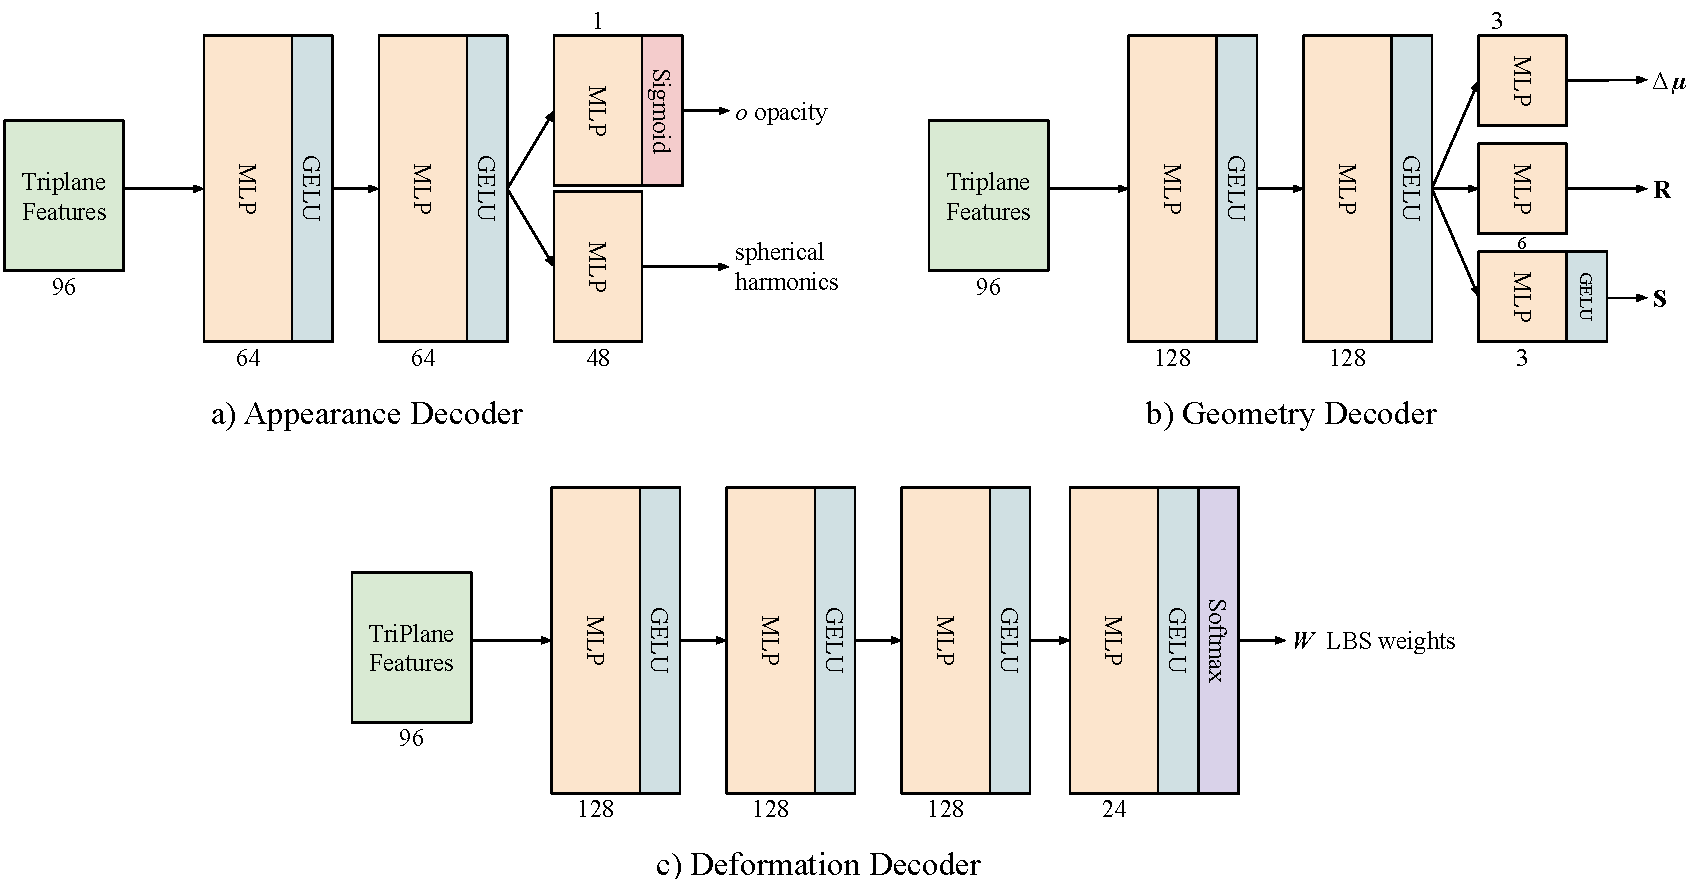
\includegraphics[width=\linewidth]{figures/pdf_files/network_architecture.pdf}
    \vspace{-7mm}
    \caption{\textbf{\acronym model architecture.} Here we show the network architecture of decoder models. 
    Appearance decoder $D_A$ is a 2-layer MLP with GELU~\cite{hendrycks2016gelu} activations. It takes triplane features as input and outputs opacity \& spherical harmonics parameters. Sigmoid activation function is used for opacity to constrain the values between $[0, 1]$. Geometry decoder $D_G$ also uses 2-layer MLP with GELU activation. It outputs the $\Delta \bm{\mu}, \bm{R}, \bm{S}$ for each Gaussians. We use GELU activation to ensure $\bm{S} \ge 0$. We do not need a normalization activation for $R$ unlike Kerbl \etal~\cite{kerbl3Dgaussians} since we use 6D rotation representation. We use a 3-layer MLP for deformation decoder $D_D$. It outputs the LBS weights. We apply a low-temperature softmax activation function with $T=0.1$ to ensure $\sum_{k=1}^{n_k} W_{k,i} = 1$. The use of a low temperature assists in predicting unimodal distributions, as most Gaussians need to be assigned to a single bone transformation.
    }
    \label{fig:netarch}
    \vspace{-2ex}
\end{figure*}{}
% We demonstrate a detailed view of the TriPlane-MLP model in \cref{fig:netarch} used to represent the human avatars. Our model use lightweight MLP models to decode the appearance, geometry, and deformation parameters of individual Gaussians. This helps us to train our model in a short amount of time without adding much overhead to the overall pipeline. We empirically found out that the GELU~\cite{hendrycks2016gelu} activation function lead to faster convergence. During rendering time Triplane and MLP models are discarded after predicting the canonical human avatar and its deformation parameters, which enables our method to perform fast rendering at 60 FPS.

We present a detailed overview of the triplane-MLP model in \cref{fig:netarch}, employed for representing human avatars. Our model utilizes lightweight MLP models to predict the appearance, geometry, and deformation parameters of individual Gaussians. This facilitates efficient model training within a short timeframe without significantly increasing the overall pipeline's computational burden. Through empirical investigation, we observed that the GELU activation function~\cite{hendrycks2016gelu} leads to quicker convergence. During the rendering phase, both triplane and MLP models are discarded once they predict the canonical human avatar and its deformation parameters. This design choice enables our method to achieve fast rendering at 60 FPS.

\paragraph{Appearance decoder ($D_A$)} comprises a 2-layer MLP with GELU activations~\cite{hendrycks2016gelu}. It takes triplane features as input and predicts opacity and spherical harmonics parameters. The opacity values are constrained within the range of $[0, 1]$ using a sigmoid activation function. Although no activation function is applied to the spherical harmonics parameters, the derived RGB values are clipped to be within $[0, 1]$ during the rasterization process.

\paragraph{Geometry decoder ($D_G$)} utilizes a 2-layer MLP with GELU activation, generating $\Delta \bm{\mu}, \bm{R}$, and $\bm{S}$ for each Gaussian. GELU activation ensures that $\bm{S} \ge 0$. Unlike Kerbl et al.~\cite{kerbl3Dgaussians}, we do not require a normalization activation for $\bm{R}$ as we employ a 6D rotation representation~\cite{Zhou_2019}.

\paragraph{Deformation decoder ($D_D$)} employs a 3-layer MLP to output LBS weights. We apply a low-temperature softmax activation function with $T=0.1$ to ensure $\sum_{k=0}^{n_k} \bm{W}_{k,i} = 1$. The use of a low temperature assists in predicting unimodal distributions, as most Gaussians need to be assigned to a single bone transformation.

\subsection{Loss implementation}
\paragraph{LBS regularization $\mathcal{L}_{\text{LBS}}$:} Given the limited set of training images, not regularizing LBS weights yields artifacts with unseen poses. Therefore, we apply regularization to ensure that the predicted LBS weights $\bm{W}$ closely align with those obtained from SMPL, employing an $\ell_2$ loss.

Specifically, to regularize the LBS weights $\bm{W}$, for individual Gaussians $\bm{p}_i$ we retrieve their $k=6$ nearest vertices on the \smpl mesh and take a distance-weighted average of their LBS weights to get $\hat{\bm{W}}$. The loss is $\mathcal{L}_{\text{LBS}} = \| \bm{W} - \hat{\bm{W}} \|_{\text{F}}^2$.

Following \cite{chen2021animatable,Zheng2020PaMIRPM} the distance-weighted average $\hat{\bm{W}_i}$ is obtained using:
\begin{align}
%\sum_{i \in \mathcal{N}(\bm{p}_i)}
    \hat{\bm{W}_i} &= \sum_{j \in \mathcal{N}_i}  \frac{\omega_j}{\omega} \bm{W}_j \label{eq:lbsquery}\\
    \omega_j &= \exp \left( {-\frac{\| \bm{p}_i - \bm{p}_j \| \| \bm{W}_i - \bm{W}_j \|}{2\sigma^2}} \right) \\
    \omega &= \sum_{j \in \mathcal{N}_i} \omega_j
\end{align}

where $\mathcal{N}_i$ is the $k$ nearest neighbor of $\bm{p}_i$. We use the efficient CUDA $k$-nn implementation of PyTorch3D library~\cite{ravi2020pytorch3d}.

% \subsection{SMPL pose parameters finetuning}
% We use off-the-shelf human pose and shape estimation models to obtain SMPL parameters. However, these models occasionally produce noisy estimates that do not align accurately with the observed human form. To address this misalignment between SMPL estimates and the actual human appearance, we incorporate joint optimization of SMPL pose parameters $\bm{\theta}$ and 3D Gaussians parameters during the training process. In Figure XXX, we illustrate the impact of online optimization on improving the accuracy of the estimates.

\subsection{Adaptive control of the number of 3D Gaussians}
We initialize the 3D Gaussians using a subdivided SMPL template with $n_v=110,210$ vertices. Despite the large number of vertices, the uniform subdivision across the body results in certain parts (e.g., face, hair, clothing) lacking sufficient points to represent high-frequency details. To address this issue, we adaptively control the number of 3D Gaussians during optimization, following a similar approach to Kerbl et al.~\cite{kerbl3Dgaussians}. The densification process starts after training the model for 3000 iterations, and subsequent densification steps are applied every 600 iterations.

% \section{Experiments}

\subsection{Ablation experiments}
\begin{figure*}[t]
    \centering
    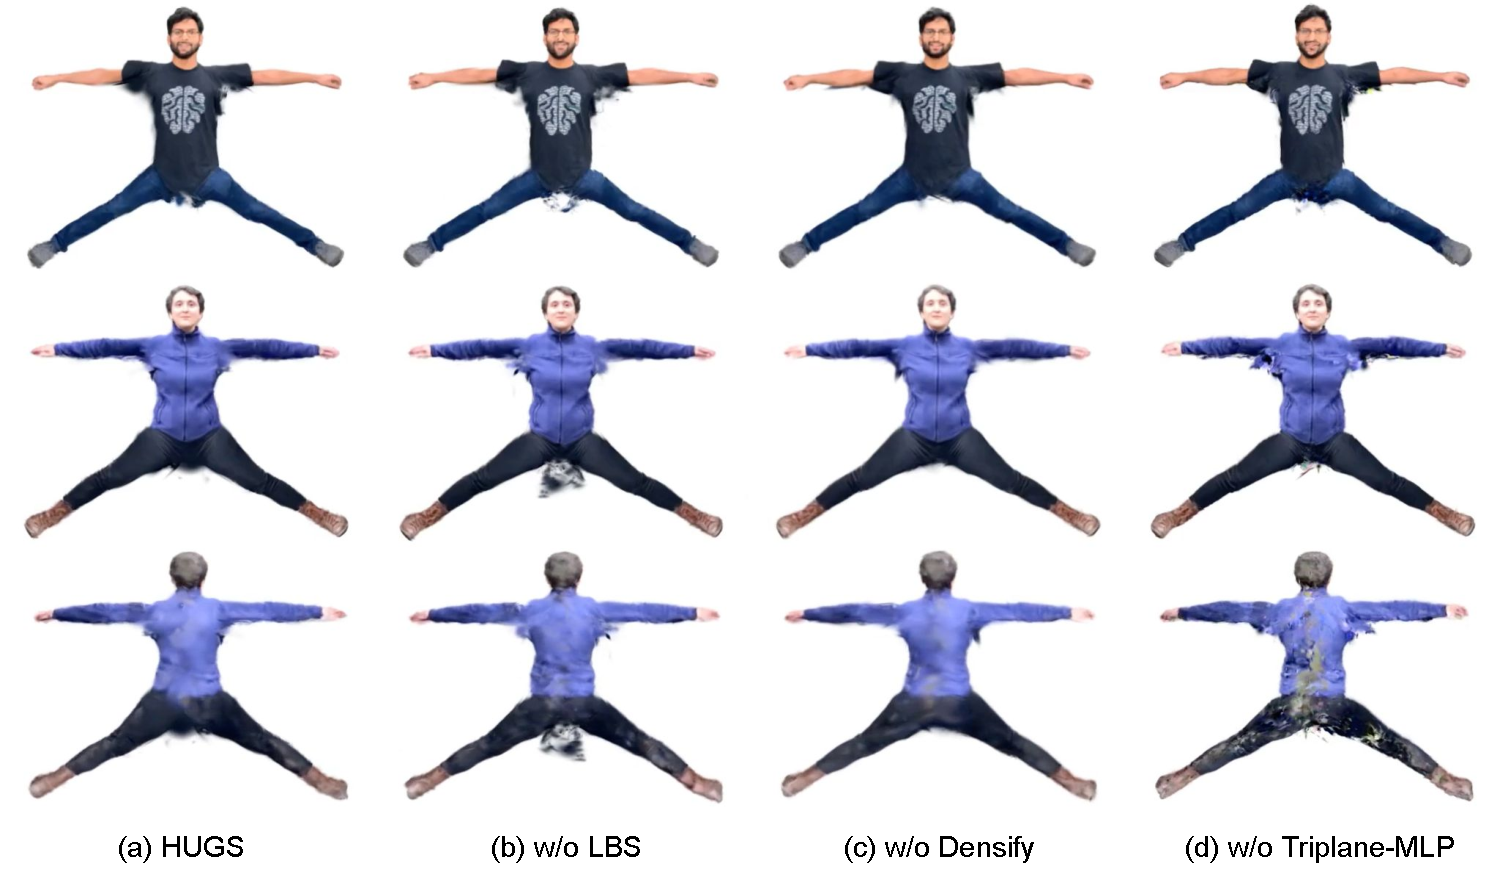
\includegraphics[width=\linewidth]{figures/pdf_files/ablation_supmat.pdf}
    \caption{\textbf{Ablation study} showing the visualization of details captured in the human canonical shape under different ablations of our method.} 
    \label{fig:ablation_supmat}
\end{figure*}

In this section, we provide a detailed explanation of the ablation experiments.

\paragraph{w/o LBS baseline.} We replace the learned LBS weights with the SMPL LBS weights to assess the significance of learnable deformation. We obtain the SMPL LBS weights for a query point $\bm{p}_i$ using \cref{eq:lbsquery}. As the $k$-nn (k-nearest neighbors) approach can be ambiguous for points around the intersection of joints, utilizing SMPL weights may result in artifacts, particularly visible in areas around these intersections, as illustrated in (a) and (b) columns in \cref{fig:ablation_supmat}.

\paragraph{w/o Densify.} In this ablation experiment, we maintain a fixed number of Gaussians throughout the optimization process. The results of this experiment are depicted in the (a) and (c) columns in \cref{fig:ablation_supmat}. The \textit{w/o Densify} setting leads to certain Gaussians protruding from the body, resulting in a suboptimal reconstruction of details, as evidenced by the example of boot laces in the second row.

\paragraph{w/o triplane-MLP baseline.} In this ablation experiment, we directly optimize the 3D Gaussian parameters instead of learning them with a trilane-MLP model. To deform individual Gaussians, we utilize the SMPL LBS weights obtained using the query algorithm presented in \cref{eq:lbsquery}. The results of this experiment are displayed in the (a) and (d) columns in \cref{fig:ablation_supmat}. As each Gaussian is optimized independently, the per-Gaussian colors have a tendency to overfit to the training frames, leading to color artifacts. This results in poor quality on novel animation renderings and test frames. On the other hand, triplane-MLP provides implicit regularization to the color as a function of Gaussian position. Also, the learned appearance provides additional 3D supervision signal for the positions of the Gaussians.

\paragraph{w/o Joint human \& scene optimization.} We assess the impact of jointly optimizing the human and scene models in this ablation experiment. Our final model, HUGS, represents human and scene Gaussians separately, however the optimization is performed jointly. An alternative approach involves initially optimizing the scene by masking out human regions and then optimizing the human Gaussians. This strategy aligns with the approach used in NeuMan~\cite{jiang2022neuman}. However, as illustrated in column (b) of \cref{fig:ablation_joint_opt}, this alternative strategy results in floating Gaussians in the scene due to sparse input views. On the contrary, when human and scene optimization is performed jointly, the human serves as a constraint for the scene reconstruction, mitigating the occurrence of floaters and yields cleaner rendered images as displayed in column (a) of \cref{fig:ablation_joint_opt}.

% We ablate the impact of jointly optimizing the human and scene models. Our final model HUGS represented human and scene Gaussians separately; however optimization is performed jointly. An alternative to this is to first optimize the scene by masking out human regions and then optimize the human Gaussians. This is the strategy employed in NeuMan~\cite{jiang2022neuman}. However as shown in \cref{fig:ablation_joint_opt} this strategy leads to floating Gaussians in the scene. This is because of sparse input views. However when jointly optimizing human and scene yields, human constrains the scene reconstruction to mitigate the floaters.
% Left is the result of optimizing the human and scene model jointly. Right is the result of optimizing the scene first and then optimizing the human model. Overall human movement helps to constrain the scene geometry. This leads to a more accurate human and scene reconstruction.

\begin{figure*}[t]
    \centering
    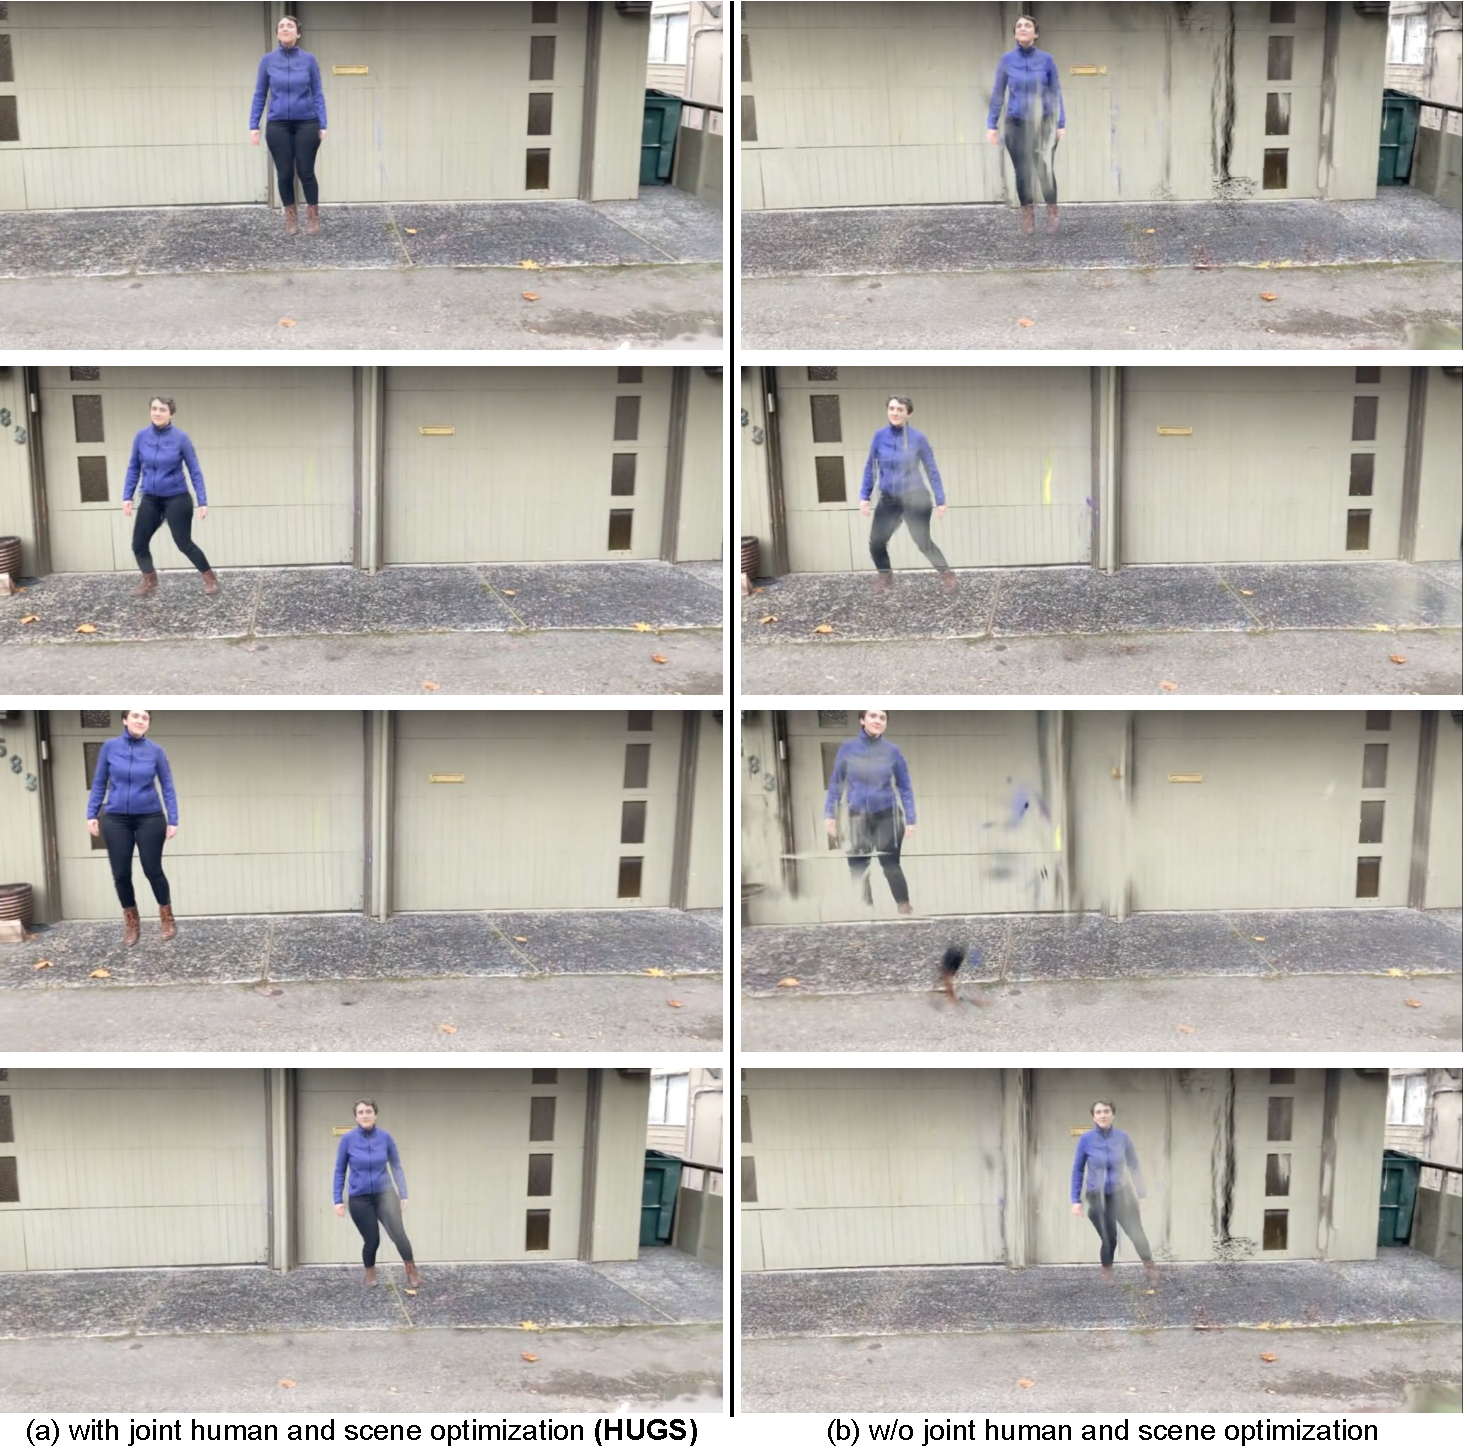
\includegraphics[width=\linewidth]{figures/pdf_files/ablation_joint_opt.pdf}
    \caption{\textbf{Ablation study} showing the impact of jointly optimizing the human and scene models. Left column (a) shows the result of our method HUGS with joint optimization of human and scene Gaussians. Right column (b) shows optimizing the scene first by masking out the human regions and then optimizing the human Gaussians.} 
    \label{fig:ablation_joint_opt}
\end{figure*}

\subsection{Novel animation renderings}

In \cref{fig:posed_renders}, we present novel animation renderings featuring subjects from the NeuMan dataset~\cite{jiang2022neuman}. Additionally, \cref{fig:novel_scene_pose} showcases the composition of multiple animated subjects in various scenes, with poses obtained from the AMASS motion capture dataset~\cite{AMASS:ICCV:2019}. For a more extensive collection of video results demonstrating novel pose and scene animations, please refer to our supplementary webpage.

\begin{figure*}[t]
    \centering
    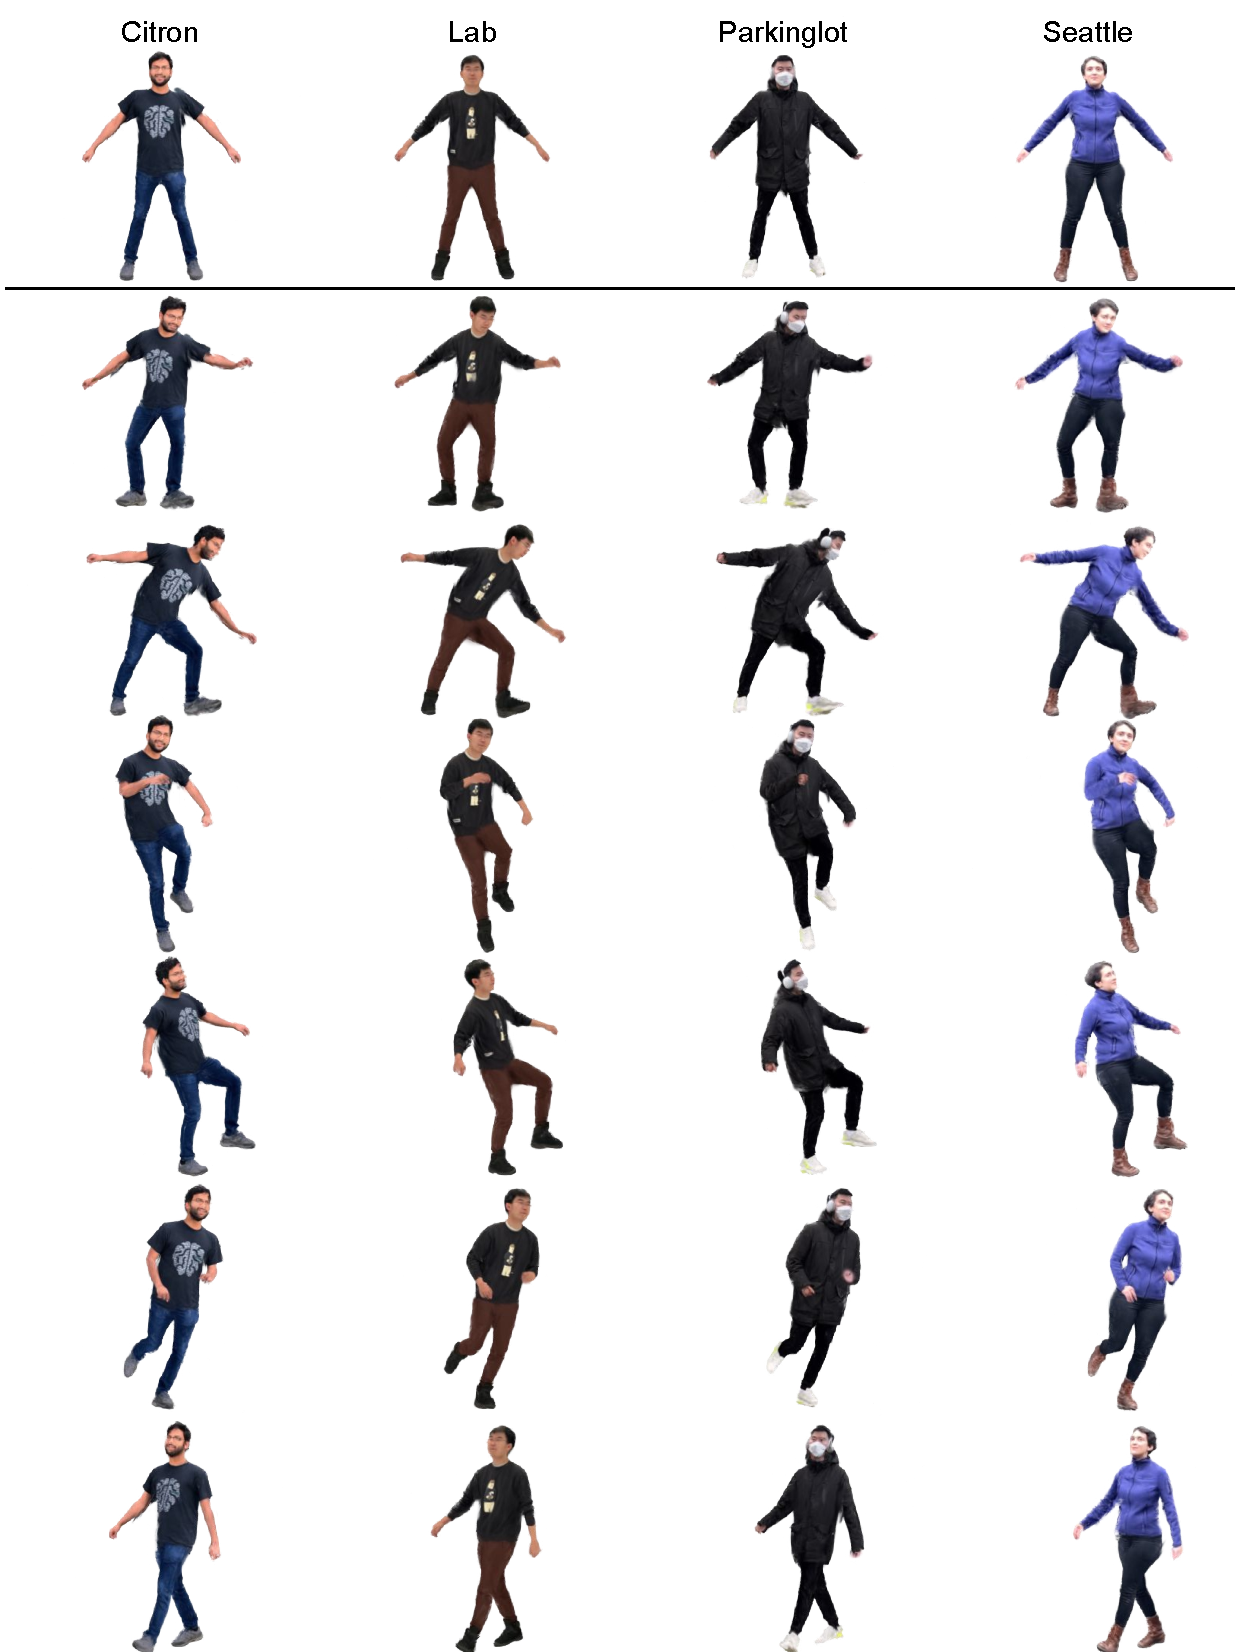
\includegraphics[width=0.9\linewidth]{figures/pdf_files/posed_imgs.pdf}
    \caption{\textbf{Novel pose renderings} We demonstrate the novel pose renderings of subjects (top row) from the NeuMan dataset.} 
    \label{fig:posed_renders}
\end{figure*}{}
\begin{figure*}[t]
    \centering
    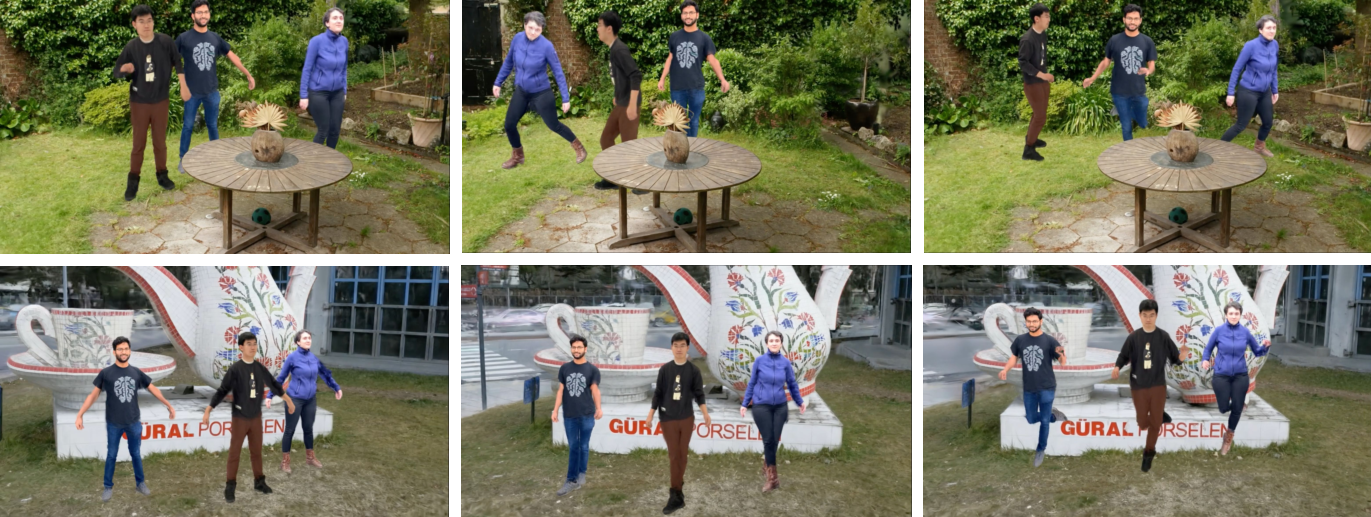
\includegraphics[width=\linewidth]{figures/pdf_files/novel_scene_pose.pdf}
    \caption{\textbf{Animation of multiple people in novel scenes.} Renderings obtained by transferring the Human Gaussians to different scenes.}
    \label{fig:novel_scene_pose}
\end{figure*}{}